

\tikzset{every picture/.style={line width=0.75pt}} %set default line width to 0.75pt        

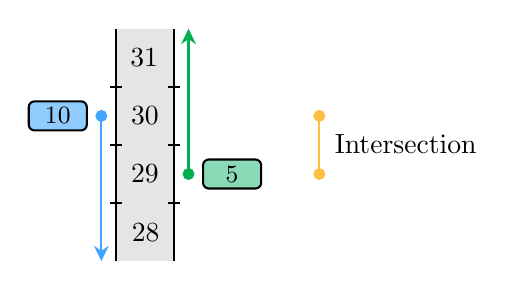
\begin{tikzpicture}[x=0.75pt,y=0.75pt,yscale=-0.7,xscale=0.7]
%uncomment if require: \path (0,300); %set diagram left start at 0, and has height of 300

%Shape: Rectangle [id:dp13563874266693043] 
\draw  [draw opacity=0][fill={rgb, 255:red, 0; green, 0; blue, 0 }  ,fill opacity=0.1 ] (230,60) -- (270,60) -- (270,220) -- (230,220) -- cycle ;
%Rounded Rect [id:dp5561959472232012] 
\draw  [fill={rgb, 255:red, 138; green, 218; blue, 184 }  ,fill opacity=1 ][line width=0.75]  (290,154) .. controls (290,151.79) and (291.79,150) .. (294,150) -- (326,150) .. controls (328.21,150) and (330,151.79) .. (330,154) -- (330,166) .. controls (330,168.21) and (328.21,170) .. (326,170) -- (294,170) .. controls (291.79,170) and (290,168.21) .. (290,166) -- cycle ;
%Straight Lines [id:da05571726881476602] 
\draw    (230,60) -- (230,220) (234,100) -- (226,100)(234,140) -- (226,140)(234,180) -- (226,180) ;
%Straight Lines [id:da7319727700794608] 
\draw    (270,60) -- (270,220) (274,100) -- (266,100)(274,140) -- (266,140)(274,180) -- (266,180) ;
%Straight Lines [id:da8116302583311774] 
\draw [color={rgb, 255:red, 0; green, 176; blue, 79 }  ,draw opacity=1 ]   (280,160) -- (280,63) ;
\draw [shift={(280,60)}, rotate = 90] [fill={rgb, 255:red, 0; green, 176; blue, 79 }  ,fill opacity=1 ][line width=0.08]  [draw opacity=0] (10.72,-5.15) -- (0,0) -- (10.72,5.15) -- (7.12,0) -- cycle    ;
\draw [shift={(280,160)}, rotate = 270] [color={rgb, 255:red, 0; green, 176; blue, 79 }  ,draw opacity=1 ][fill={rgb, 255:red, 0; green, 176; blue, 79 }  ,fill opacity=1 ][line width=0.75]      (0, 0) circle [x radius= 3.35, y radius= 3.35]   ;
%Straight Lines [id:da8103839365180321] 
\draw [color={rgb, 255:red, 65; green, 165; blue, 255 }  ,draw opacity=1 ]   (220,120) -- (220,217) ;
\draw [shift={(220,220)}, rotate = 270] [fill={rgb, 255:red, 65; green, 165; blue, 255 }  ,fill opacity=1 ][line width=0.08]  [draw opacity=0] (10.72,-5.15) -- (0,0) -- (10.72,5.15) -- (7.12,0) -- cycle    ;
\draw [shift={(220,120)}, rotate = 90] [color={rgb, 255:red, 65; green, 165; blue, 255 }  ,draw opacity=1 ][fill={rgb, 255:red, 65; green, 165; blue, 255 }  ,fill opacity=1 ][line width=0.75]      (0, 0) circle [x radius= 3.35, y radius= 3.35]   ;
%Rounded Rect [id:dp6586100738433943] 
\draw  [fill={rgb, 255:red, 143; green, 203; blue, 253 }  ,fill opacity=1 ][line width=0.75]  (170,114) .. controls (170,111.79) and (171.79,110) .. (174,110) -- (206,110) .. controls (208.21,110) and (210,111.79) .. (210,114) -- (210,126) .. controls (210,128.21) and (208.21,130) .. (206,130) -- (174,130) .. controls (171.79,130) and (170,128.21) .. (170,126) -- cycle ;
%Straight Lines [id:da4565659656057395] 
\draw [color={rgb, 255:red, 255; green, 191; blue, 65 }  ,draw opacity=1 ]   (370,120) -- (370,160) ;
\draw [shift={(370,160)}, rotate = 90] [color={rgb, 255:red, 255; green, 191; blue, 65 }  ,draw opacity=1 ][fill={rgb, 255:red, 255; green, 191; blue, 65 }  ,fill opacity=1 ][line width=0.75]      (0, 0) circle [x radius= 3.35, y radius= 3.35]   ;
\draw [shift={(370,120)}, rotate = 90] [color={rgb, 255:red, 255; green, 191; blue, 65 }  ,draw opacity=1 ][fill={rgb, 255:red, 255; green, 191; blue, 65 }  ,fill opacity=1 ][line width=0.75]      (0, 0) circle [x radius= 3.35, y radius= 3.35]   ;

% Text Node
\draw (250,119.5) node    {$30$};
% Text Node
\draw (310,160) node  [font=\small]  {${\textstyle 5}$};
% Text Node
\draw (250,160) node    {$29$};
% Text Node
\draw (250.5,200) node    {$28$};
% Text Node
\draw (249.5,80) node    {$31$};
% Text Node
\draw (190,120) node  [font=\small]  {$10$};
% Text Node
\draw (429.5,139.5) node   [align=left] {Intersection};


\end{tikzpicture}
